%% bare_conf.tex
%% V1.3
%% 2007/01/11
%% by Michael Shell
%% See:
%% http://www.michaelshell.org/
%% for current contact information.
%%
%% This is a skeleton file demonstrating the use of IEEEtran.cls
%% (requires IEEEtran.cls version 1.7 or later) with an IEEE conference paper.
%%
%% Support sites:
%% http://www.michaelshell.org/tex/ieeetran/
%% http://www.ctan.org/tex-archive/macros/latex/contrib/IEEEtran/
%% and
%% http://www.ieee.org/

%%*************************************************************************
%% Legal Notice:
%% This code is offered as-is without any warranty either expressed or
%% implied; without even the implied warranty of MERCHANTABILITY or
%% FITNESS FOR A PARTICULAR PURPOSE! 
%% User assumes all risk.
%% In no event shall IEEE or any contributor to this code be liable for
%% any damages or losses, including, but not limited to, incidental,
%% consequential, or any other damages, resulting from the use or misuse
%% of any information contained here.
%%
%% All comments are the opinions of their respective authors and are not
%% necessarily endorsed by the IEEE.
%%
%% This work is distributed under the LaTeX Project Public License (LPPL)
%% ( http://www.latex-project.org/ ) version 1.3, and may be freely used,
%% distributed and modified. A copy of the LPPL, version 1.3, is included
%% in the base LaTeX documentation of all distributions of LaTeX released
%% 2003/12/01 or later.
%% Retain all contribution notices and credits.
%% ** Modified files should be clearly indicated as such, including  **
%% ** renaming them and changing author support contact information. **
%%
%% File list of work: IEEEtran.cls, IEEEtran_HOWTO.pdf, bare_adv.tex,
%%                    bare_conf.tex, bare_jrnl.tex, bare_jrnl_compsoc.tex
%%*************************************************************************

% *** Authors should verify (and, if needed, correct) their LaTeX system  ***
% *** with the testflow diagnostic prior to trusting their LaTeX platform ***
% *** with production work. IEEE's font choices can trigger bugs that do  ***
% *** not appear when using other class files.                            ***
% The testflow support page is at:
% http://www.michaelshell.org/tex/testflow/



% Note that the a4paper option is mainly intended so that authors in
% countries using A4 can easily print to A4 and see how their papers will
% look in print - the typesetting of the document will not typically be
% affected with changes in paper size (but the bottom and side margins will).
% Use the testflow package mentioned above to verify correct handling of
% both paper sizes by the user's LaTeX system.
%
% Also note that the "draftcls" or "draftclsnofoot", not "draft", option
% should be used if it is desired that the figures are to be displayed in
% draft mode.
%
\documentclass[a4paper]{IEEEtran}
\pagestyle{empty}

% Add the compsoc option for Computer Society conferences.
%
% If IEEEtran.cls has not been installed into the LaTeX system files,
% manually specify the path to it like:
% \documentclass[conference,a4paper]{../sty/IEEEtran}


% Some very useful LaTeX packages include:
% (uncomment the ones you want to load)

% *** MISC UTILITY PACKAGES ***
%
%\usepackage{ifpdf}
% Heiko Oberdiek's ifpdf.sty is very useful if you need conditional
% compilation based on whether the output is pdf or dvi.
% usage:
% \ifpdf
%   % pdf code
% \else
%   % dvi code
% \fi
% The latest version of ifpdf.sty can be obtained from:
% http://www.ctan.org/tex-archive/macros/latex/contrib/oberdiek/
% Also, note that IEEEtran.cls V1.7 and later provides a builtin
% \ifCLASSINFOpdf conditional that works the same way.
% When switching from latex to pdflatex and vice-versa, the compiler may
% have to be run twice to clear warning/error messages.


% *** CITATION PACKAGES ***
%
\usepackage{cite} 
% cite.sty was written by Donald Arseneau
% V1.6 and later of IEEEtran pre-defines the format of the cite.sty package
% \cite{} output to follow that of IEEE. Loading the cite package will
% result in citation numbers being automatically sorted and properly
% "compressed/ranged". e.g., [1], [9], [2], [7], [5], [6] without using
% cite.sty will become [1], [2], [5]--[7], [9] using cite.sty. cite.sty's
% \cite will automatically add leading space, if needed. Use cite.sty's
% noadjust option (cite.sty V3.8 and later) if you want to turn this off.
% cite.sty is already installed on most LaTeX systems. Be sure and use
% version 4.0 (2003-05-27) and later if using hyperref.sty. cite.sty does
% not currently provide for hyperlinked citations.
% The latest version can be obtained at:
% http://www.ctan.org/tex-archive/macros/latex/contrib/cite/
% The documentation is contained in the cite.sty file itself.


% *** GRAPHICS RELATED PACKAGES ***
%
%\ifCLASSINFOpdf
  \usepackage[pdftex]{graphicx}
  % declare the path(s) where your graphic files are
  \graphicspath{{./eps}{./png}}
  % and their extensions so you won't have to specify these with
  % every instance of \includegraphics
  % \DeclareGraphicsExtension 
  % or other class option (dvipsone, dvipdf, if not using dvips). graphicx
  % will default to the driver specified in the system graphics.cfg if no
  % driver is specified.
  % \usepackage[dvips]{graphicx}
  % declare the path(s) where your graphic files are
  % and their extensions so you won't have to specify these with
  % every instance of \includegraphics
% \DeclareGraphicsExtensions{.eps}
%\fi
% graphicx was written by David Carlisle and Sebastian Rahtz. It is
% required if you want graphics, photos, etc. graphicx.sty is already
% installed on most LaTeX systems. The latest version and documentation can
% be obtained at: 
% http://www.ctan.org/tex-archive/macros/latex/required/graphics/
% Another good source of documentation is "Using Imported Graphics in
% LaTeX2e" by Keith Reckdahl which can be found as epslatex.ps or
% epslatex.pdf at: http://www.ctan.org/tex-archive/info/
%
% latex, and pdflatex in dvi mode, support graphics in encapsulated
% postscript (.eps) format. pdflatex in pdf mode supports graphics
% in .pdf, .jpeg, .png and .mps (metapost) formats. Users should ensure
% that all non-photo figures use a vector format (.eps, .pdf, .mps) and
% not a bitmapped formats (.jpeg, .png). IEEE frowns on bitmapped formats
% which can result in "jaggedy"/blurry rendering of lines and letters as
% well as large increases in file sizes.
%
% You can find documentation about the pdfTeX application at:
% http://www.tug.org/applications/pdftex

% *** MATH PACKAGES ***
%
\usepackage[utf8]{inputenc}
\usepackage[cmex10]{amsmath}
\usepackage{amssymb}

\usepackage{float}

\usepackage{url}


\usepackage[top=2.4cm,left=1.5cm,right=1.5cm,bottom=3.5cm]{geometry}

% Set dimensions of columns, gap between columns, and paragraph indent
%\setlength{\textheight}{8.875in} \setlength{\textwidth}{6.875in}
\setlength{\columnsep}{0.24in} %\setlength{\topmargin}{0in}
%\setlength{\headheight}{0in} 
\setlength{\headsep}{0in}
\setlength{\parindent}{1.2pc}
%\setlength{\oddsidemargin}{-.1875in}  % Centers text.
%\setlength{\evensidemargin}{-.1875in}

% Add the period after section numbers.  Adjust spacing.
%\newcommand{\Section}[1]{\vspace{-8pt}\section{\hskip -1em.~~#1}\vspace{-3pt}}
%\newcommand{\SubSection}[1]{\vspace{-3pt}\subsection{\hskip -1em.~~#1}
 %       \vspace{-3pt}}
				
\begin{document}

%
% paper title
% can use linebreaks \\ within to get better formatting as desired
\title{Electromagnetic Characterisation of a Short-\\ Stroke Ferromagnetic Actuator Technical Note\vspace{-.1em}}

\author{Bowen Zhang, \textit{1975667}
	and Weifeng Du, \textit{1975663}
\vspace{-.45em}
}

% make the title area
\maketitle

\thispagestyle{empty}
\begin{abstract}
The electromagnetic actuators are widely used in automotive, industrial automation and protection system\cite{applications}. 
In this article, a model was built using MATLAB and FEMM in order to 
analyse the characterization of an actuator and the comparison between different analyzing methods is made. 
The principle of a short-stroke ferromagnetic actuator is discussed 
and 4 different modelling approaches used to model the actuator are compared. In addition, the resistance, inductance of the actuator and force imparted on mover of the actuator are discussed in this article.
It has been found that FEMM simulation tools using non-linear core produces the most 
accurate result.
\end{abstract}

\vspace{1em}



\section{Introduction}
This technical note incorporates the calculations of the winding resistance, winding inductance 
of a Short-Stroke Ferromagnetic Actuator depicted in Fig. 1 and the finding on 
the force imparted on the Armature. Four different modelling 
approaches are used with the intention of finding the inductance of the actuator and force imparted on the mover
(i.e. analytical equivalent circuit without considering air-gap 
fringing, analytical equivalent circuit with air-gap fringing, 
FEMM with linear materials and FEMM with non-linear materials\cite{notes_b}). 
The modelling method discussed in this technical note is Finite Element 
Method Magnetic (FEMM), which plays a critical role in discipline of electromagnetic field.
The Finite Element Method(FEM) emerges in different disciplines such as biology\cite{biology_application}, civil engineering\cite{civil_application} and dynamics\cite{dynamics_application}
MATLAB and FEMM are used for more precise and faster calculations.

\section{Winding Resistance}
\subsection{The Winding resistance calculated using voltage and current measured by FEMM}                  
FEMM and MATLAB can be readily used to calculate the winding resistance. 
This can be achieved by using command \textit{mo\textunderscore getcircuitproperties()} to calculate the current $I$ and voltage $V$ in the coil.
Then the resistance could be found using \eqref{ohms law}
\begin{equation}
R_w=\frac{V_w}{I_w} \label{ohms law}
\end{equation}
According to the data collected from FEMM model, the voltage and current on a single coil is $V_w=0.1066\hskip 0.2em\text{V}$
and $I_w=10\hskip 0.2em\text{A}$, the resistance could be calculated using \eqref{ohms law}, which yields the single winding resistance $R_{w}$=10.66$\hskip 0.2emm\Omega$.
\subsection{The Winding resistance calculated using effective length measured by FEMM}
Another approach is to use \eqref{effective length} to calculate the effective length $l_w$.
Thus, it would be possible to calculate the $R_w$ with the definition of resistance described in \eqref{resistance formula}\cite{notes_a}
\begin{equation}%{align}
l_w=\frac{V_w}{A_w} \label{effective length}
\end{equation}
\begin{equation}
R_w=\frac{Nl_w}{\sigma((k_{PF})A_w)/N} \label{resistance formula}
\end{equation}
The volumeof coil $V_w$ and the area of the cross-section $A_w$ could be measured by
the FEMM, which are $V_w= 1.29\times10^{-5}\hskip 0.2em m^3$ and $A_w=6.48\times10^{-4}\hskip 0.2em m^2$.
Substitute them into \eqref{effective length}, the effective length $l_w$ could be found, which is 
$l_w=2\hskip 0.2em\text{cm}$. Then if substitute $l_w=2\hskip 0.2em\text{cm}$, $N=100\hskip 0.2em\text{turns}$, 
$\sigma=58 \hskip 0.2em\text{MS/m}$, $k_{PF}=0.6$ and $A_w=6.48\times10^{-4}\hskip 0.2em m^2$ into \eqref{resistance formula}, 
it is readily to find the resistance of a half of a winding is $R_{halfwinding}=8.896\hskip 0.2emm\Omega$. Both two windings
comprise 2 of the half winding. Thus, the total resistance of one winding is $R_{w}=17.79\hskip 0.2emm\Omega$.
\subsection{The Winding resistance calculated using CAD model}
However, the FEMM model used in simulation is a 2D model, which omits more than a
half of the coil in simulation. In the light of this, as shown in Fig. 1, a CAD model is introduced in order to find the actual resistance
of the coil. To find the total resistance of a single coil, the actual length of winding needs to be found.
Through calculations
with the help of the 3D CAD model, it could be readily found that the total length of wire in one single coil is $l_{total}=12346.9\hskip 0.2em\text{mm}$.
Substitute the value of $l_{total}$, i.e. $l_w$, into \eqref{resistance formula} and the resistance of one single winding could be found,
which is $R_{w}=55.7\hskip 0.2emm\Omega$.
\begin{figure}[!ht]
\begin{centering}
\includegraphics[scale=0.8]{CAD_model_of_actuator.jpg}
\par\end{centering}   
\caption{The 3D CAD model of the actuator.\label{CAD model of actuator}}
\end{figure}   

\subsection{Compare the analytical result and that calculated using the measured voltage and current reported from FEM model}
It can be seen that the resistance that is calculated by analytical method is slightly bigger than that calculated by 
the measured current and voltage. The probable reason is that the packing factor is different. It can be readily seen the 
winding material property is the same in the FEMM property option. The electrical conductivity the software uses to calculate the 
resistance is the same as ours, which is $\sigma=58 \hskip 0.2em\text{MS/m}$. However, FEMM uses a unity packing factor (i.e. $k_{PF}=1$).
This should be the reason why we get a different result from our calculations and simulations.

\subsection{Plot the total winding loss as a function of applied current from 0 to 10A}
In this case, the current is DC current. Thus, we may consider the resistance to be constant when the current $I$ range from
$0\hskip 0.2emA$ to $10\hskip 0.2emA$. With the intention of finding the most accurate result, it is appropriate to use the resistance calculated using CAD model, which is $R_w=55.7\hskip 0.2emm\Omega$.
The power loss in winding is governed by \eqref{power}. It is readily to use MATLAB to plot the total winding power loss as shown in Fig. 2.

\begin{equation}
  P=I^2R\label{power}
\end{equation}

\begin{figure}[H]
\begin{centering}
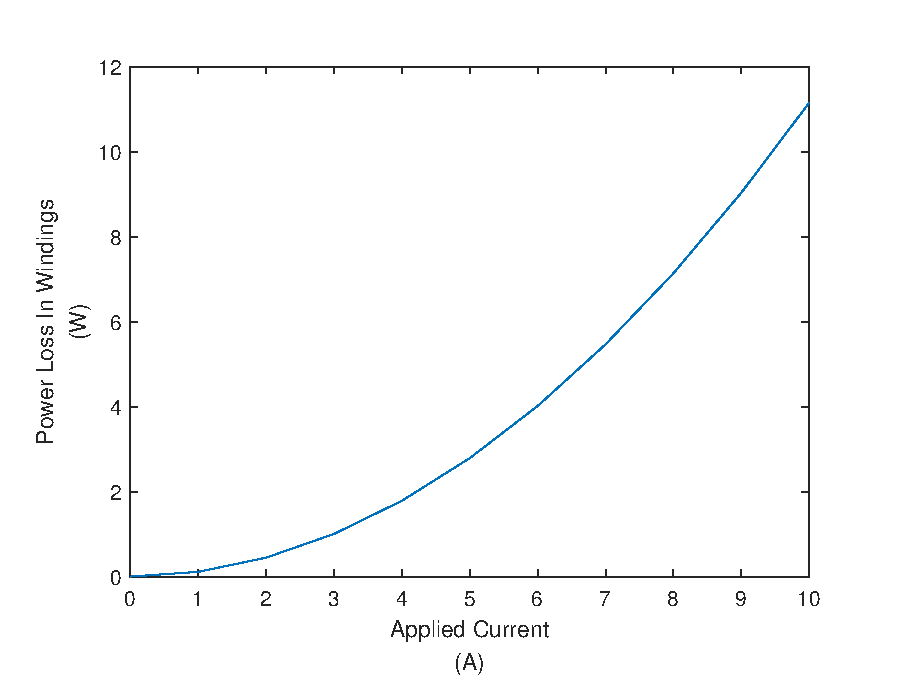
\includegraphics[scale=0.55]{P-I.eps}
\par\end{centering}   
\caption{Total windings (including all 2 windings) Power Loss $P$ v.s. Applied Current $I$ ranging from 0A to 10A.\label{power loss in winding vs. applied current}}
\end{figure}   

%-----------------------------------------------------------------------------------------
%-----------------------------------------------------------------------------------------
%-----------------------------------------------------------------------------------------
\section{Winding Inductance}
In this section, only the half-side inductance is considered because the same turns of coil and current on each side sets up the same magneto-motive force, hence the performance of both sides are symmetrical. 
The figures of 2D model of the actuator is depicted in Fig. \ref{a} and equivalent magnetic circuit is depicted in Fig. \ref{b}
\begin{figure}[H]
\begin{centering}
\includegraphics[scale=0.7]{a.jpg}
\par\end{centering}   
\caption{The half-side actuator from FEMM.\label{a}}
\end{figure}  

\begin{figure}[H]
\begin{centering}
\includegraphics[scale=0.4]{b.jpg}
\par\end{centering}   
\caption{The half-side actuator equivalent circuit from FEMM.\label{b}}
\end{figure}   
In this scenario, $ R_{a1} $ is the reluctance of the air-gap between the stator core and the armature on the left-hand-side of Fig. \ref{a}, 
$ R_{a2} $ is the reluctance of  the air-gap between armature and core on the right handside of Fig. \ref{a}, 
$ R_{c1} $ is the reluctance of the half-side core and $ R_{c2} $ is the reluctance of the half-side armature. 
The magnetomotive force is generated by 100 turns of coil and 10A current.
Assuming the displacement from the original position of the armature is x, then the length of the air-gap is also x.\par 
From the 2D model of the actuator, some required values that are measured by FEMM are described as follows.
\begin{align}
	&\text {The flux length of the half-side stator coil:}\notag \\ 
	&l_{c1} = 150mm\\
	&\text {The flux length of the affected half-side armature:}\notag \\
	&l_{c2} = (70 - x) mm\\
	&\text{The flux length of air-gap on the left:}\notag\\
	&l_{a1} = 0.5mm\\
	&\text{The flux length of air-gap on the right:}\notag\\
	&l_{a2} = x\quad mm\\
	&\text{The effective gap area of linear condition:}\notag\\
	&A = 400 mm^2
\end{align}
The reluctance is defined as \eqref{reluctance definition}, where $l$ is the path length
$\mu_0$ is the vacuum permeability, $\mu_r$ is the relative permeability and $A$ is the surface.
\begin{equation}
  R = \frac{l}{\mu_0 \mu_r A}\label{reluctance definition}
\end{equation} 
Then the reluctances of the linear condition could then be found as below.
\begin{align}
	R_{a1} &= \frac{l_{a1}}{\mu_0 A} = \frac{0.5\times10^{-3}}{4\pi\times10^{-7}\times 400\times 10^{-6}}\notag\\ &= 9.95\times10^{5}(At/Wb)\\
	R_{a2} &= \frac{x}{\mu_0 A} = \frac{x\times 10^{-3}}{4\pi\times 10^{-7}\times 400\times 10^{-6}}\notag\\ &= 1.99\times 10^{-6}x(At/Wb)\\
	R_{c1} &= \frac{l_{c1}}{\mu_0\mu_rA} = \frac{150\times10^{-3}}{4\pi\times 10^{-7}\times 1000\times 400\times 10^{-6}}\notag\\ &= 2.98\times 10^{5} (At/Wb)\\
	R_{c2} &= \frac{l_{c2}}{\mu_0\mu_rA} = \frac{(70 + x) *10^{-3}}{4\pi\times10^{-7}\times 400\times 10^{-6}}\notag\\ &= (1.39\times 10^5 + 1.99\times 10^3x)(At/Wb)
\end{align}
And the summation of all reluctances is 
\begin{align}
	\Sigma R &= R_{a1} + R_{a2} + R_{c1} + R_{c2}\notag\\
	 &= (1.432\times 10^6 + 1.99\times 10^6x) (At/Wb) \label{noair}
\end{align}
The relation between inductance and reluctance is governed by
\begin{align}
	L = \frac{N^2}{\Sigma R} \label{firind}
\end{align} 
By substituting total reluctance (\ref{noair}) into (\ref{firind}) we can get the inductance when the air-gap fringing is negligible.
\begin{align}
	L = \frac{10^4}{1.432\times 10^6 + 1.99\times 10^6x} (H) \label{inductance not considering aeff}
\end{align}
As for the scenario when accounting for air-gap fringing flux, using the effective air-gap model that given in \cite{notes_course}.
\begin{align}
	A_{eff} = (W+2g)(T+2g) = (20+2x)(20+2x)\label{Aeff}
\end{align}
By replacing A with (\ref{Aeff}), the reluctances considering the air fringing could be calculated as in \eqref{formula1}.
\begin{align}
	R_{a1} &= \frac{l_{a1}}{\mu_0 A_{eff}} = \frac{0.5\times 10^{-3}}{4\pi\times10^{-7}\times (20+1)(20+1)\times 10^{-6}}\notag\\
  &= 9.02\times 10^5 (At/Wb) \label{formula1}
\end{align}
\begin{equation}
	R_{a2} = \frac{x}{\mu_0 A_{eff}}  
\end{equation}
\begin{equation}
	R_{a2} = \frac{10^{-3}x}{4\pi\times10^{-7}\times (20+2x)(20+2x)\times 10^{-6}}
\end{equation}
\begin{equation}
	R_{a2} = \frac{7.96\times 10^8 x}{(20+2x)(20+2x)} (At/Wb)
\end{equation}
Then we get the summation of all reluctances, which is shown as in \eqref{formula2}.
\begin{align}
	\Sigma R = 1.339\times 10^6 + 1.99\times 10^3x\notag\\ + \frac{7.96\times 10^8 x}{(20+2x)(20+2x)}  (At/Wb) \label{formula2}
\end{align}
Hence the inductance considering the air fringing could be calculated by \eqref{inductance considering aeff}.
\begin{align}
	L = \frac{10^4}{1.339\times 10^6 + 1.99\times 10^3x + \frac{7.96\times 10^8 x}{(20+2x)(20+2x)}} (H) \label{inductance considering aeff}
\end{align}

Using the FEMM model, the inductance of the actuator as a function of armature position for both the $ core\_{linear} $  and $ core\_{nonlinear} $ material cases could be readily found.
The four inductance trends is shown in Fig. \ref{induc1}.\par 

\begin{figure}[H]
\begin{centering}
\includegraphics[scale=0.4]{induc1.jpg}
\par\end{centering}   
\caption{The inductance trend plotted using four different methods.\label{induc1}}
\end{figure}   

From the Fig. {\ref{induc1}, it could be found that when the air-gap gets smaller the inductance will increase and slope of the curves will also rise. 
The reason for that is the inductance is inversely proportional to the reluctance which is proportional to the length of air-gap.
Hence, the inductance is reversely proportional to the length of air-gap.\par

Comparing the trends of the inductance with air-gap considered and without air-gap considered which are the green one and the red one respectively from Fig. {\ref{induc1}}, 
it could be found that the curve of the trend of the inductance calculated without considering air-gap fringing is smaller than that calculated with air-gap in that the air-gap induces the effective air-gap area $A_{eff}$ which makes the air-gap area larger. 
But the differences will get smaller as the air-gap gets smaller. Then a conclusion could be drawn that the air-gap fringing will make a large difference when the air-gap is too large to neglect and vice versa.
The inductance trend measured by FEMM using linear core will be compared with that plotted using the analytical method considering the effective air-gap area $A_{eff}$,
because they are both using linear core, the relative permeability $\mu_r$ should be the same. Thus, the only difference could be the effective air-gap area $A_{eff}$. We can see from the Fig. {\ref{induc1}}, when the air-gap is large, 
the inductance of the analytical method considering Aeff is larger than the numerical method either using linear core or using nonlinear core as the result of the fact that the effective air-gap area $A_{eff}$ is not accurate. The effective air-gap area $A_{eff}$ is calculated
by using the formula described in \eqref{Aeff}, which is only an approximate of the real effective air-gap area $A_{eff}$. Due to the fact that the inductance calculated by our analytical method is slightly bigger than the real one,
it could be readily seen that the effective air-gap area $A_{eff}$ calculated is slightly bigger than the one in reality since inductance $L$ is proportional to the effective air-gap area $A_{eff}$.
That is the reason why when the air-gap is large, the inductance calculated using the analytical method considering Aeff is larger than the numerical ones while the linear core and nonlinear core have the same performance.\par
\begin{figure}[H]
\centering
\includegraphics[scale=0.4]{BH.jpg}
\caption{The B-H curve and hysteresis loop of the nonlinear ferromagnetic material\label{BH}}\par
\end{figure} 
When the air-gap length is decreasing, it could be seen that the numerical-linear-core curve is drawn closer to the analytical-method-considering-Aeff one.
This is because as the reluctance decreasing, 
the effective air-gap area $A_{eff}$ is getting more accurate.
As for the nonlinear one, while the air-gap length becomes smaller, which is between 0.25mm to 5mm,
Thus, the relative permeability of the nonlinear core $\mu_r$ gets larger as the slope of B-H curve increases.
Hence its inductance is higher than the linear one during the period when air-gap is between 0.25mm and 5mm. 

Nevertheless, it could be found that when the air-gap is smaller than about 0.4mm, 
the slope of the inductance trend with a nonlinear core is slower and finally the inductance becomes smaller than the analytical 
and the linear one. This is because the nonlinear gets saturated, in other words, the relative permeability $\mu_r$ decreases, 
when the flux density gets higher Fig. {\ref{BH}}. 
From the equation \eqref{BBH}, because the slope of B-H curve,
which is equal to permeability, is getting smaller than 
the relative permeability plummets. 
Hence the inductance is also smaller compared with the other two curves.\par
 
\begin{align}
B = \mu_0\mu_rH \label{BBH}
\end{align}

\section{Simplified circuit model for nonlinear core}
Based on the previous analysis, the analytical method could not be used to model the actuator with a nonlinear core material\cite{notes_b}.
In order to solve this problem, Simulink is used to build a equivalent circuit for the nonlinear core.
The equivalent circuit model for nonlinear core could be built using a nonlinear resistance.
In this scenario, the current controlled resistor is introduced so that the relation between B and H
could be found, which is the same as the voltage-current relation in the equivalent circuit.
Based on the equation described in \eqref{BBH}, let's assume that the current $I$ corresponds to magnetic flux $\varphi$ and that voltage $U$
corresponds to magneto-motive force $NI$. Thus, the equation described in \eqref{BBH} could be transformed in to following equations.
 
\begin{align}
	\frac{\varphi}{S} = \mu_0\mu_r \frac{NI}{l} 
\end{align}
\begin{align}
	NI=\frac{l}{\mu_0\mu_r(\varphi)S}\cdot\varphi \label{BBH}
\end{align}
The equation in \eqref{BBH} is in line with the equation in \eqref{ccr}.
\begin{equation}
	U=R(I)\cdot I \label{ccr}
\end{equation}
In the light of this, a model could be built in Simulink with the \emph{Simscape} tool box\cite{Simscape}, which is shown in Fig. \ref{Simulink}.

\begin{figure}[H]
\begin{centering}
\includegraphics[scale=0.5]{Simulink.jpg}
\par\end{centering}   
\caption{Simulink model for the equivalent circuit of the nonlinear core.\label{Simulink}}
\end{figure}  

As shown in Fig. \ref{Simulink}, a current controlled resistor is used to emulate the behaviour of a nonlinear core.
It is critical to decide the resistance $R$ function w.r.t current $I$. In the light of \cite{Simscape_Electrical}, the relation between B and H in nonlinear scenario
could be define as \eqref{bhrelation}.

\begin{equation}
	B = B_{sat}\cdot tanh(a\cdot H) \label{bhrelation}
\end{equation}
where $B_{sat} = 1.5$, $a=tanh^{-1}(0.5)\cdot \frac{\mu_0\mu_r}{0.75}$. 
Thus, the derivative of magneto-motive force $NI$ w.r.t the magnetic flux $\varphi$ could be found, which is governed by \eqref{derivative of mmf}.

\begin{equation}
	\frac{dNI}{d\varphi}=\frac{d}{d\varphi}\left[\frac{l}{a} tanh^{-1}(\frac{\varphi}{s\cdot 1.5})\right] = \frac{l}{a}\cdot \frac{1}{1-((\frac{\varphi}{1.5S}))^2}\label{derivative of mmf}
\end{equation}

Then, all the parameters and formulae could be fed into MATLAB and a B-H curve could be generated through a x-y scope\cite{Simscape_Electrical}, as shown in Fig. \ref{BHcurve}.
It could readily be seen that the BH curve is linear when M.M.F $NI$ is not greater than 40.
If M.M.F $NI$ goes greater than 40, the nonlinear characteristic of nonlinear core is shown as these curves.
In addition, the parameters used in this example could be altered easily in order to apply to different demands.

\begin{figure}[H]
\begin{centering}
\includegraphics[scale=0.35]{BHcurve.jpg}
\par\end{centering}   
\caption{B-H curve plotted using Simulink and MATLAB.\label{BHcurve}}
\end{figure}  

\section{Force on the Armature}
If not specified, the following calculations and measurements are all based on the assumption that only one single winding is considered.
\subsection{Using FEMM method to find the $\psi-I$ relation}
It could be easily seen that the force varies as the mover of the
actuator moving from the closed position to the open position. In order 
to take the advantage of the actuator, it is critical to find how force varies when
the mover is changing its position. The force could be assessed through an 
energy conservation perspective. The relation between force imparted on the mover
and the displacement of the mover is governed by \eqref{f-x relation} [1]
\begin{equation}
  \Delta E_{mech}=\int_{dx_0}^{dx_c}  \,F\mathrm{d}x \label{f-x relation}
\end{equation}
In order to find the relation between force imparted on the mover and displacement of mover,
the difference of mechanical energy $\Delta E_{mech}$ must be found.
From the conclusion derived in [2], it could be readily found that the difference of Coenergy is the 
mechanical energy $\Delta E_{mech}$ that is looked for, which could be seen from the
$\psi-I$ diagrams. Take Fig. {\ref{psi-i_nonlinear}} as an example, the $\psi-I$ relation is governed by
\eqref{f formula}.

\begin{figure}[H]
\begin{centering}
\includegraphics[scale=0.3]{psi-i_nonlinear.jpg}
\par\end{centering}   
\caption{$\psi-I$ plot with nonlinear core in 10 different positions.\label{psi-i_nonlinear}}
\end{figure}  

\begin{equation}
  F=\frac{\Delta E_{mech}}{\Delta x} \label{f formula}
\end{equation}

It could also be seen in Fig. \ref{psi-i_nonlinear} that the difference of mechanical energy could be calculated
by the area encircled by two corresponding curves. Therefore, we could just calculate the area between two curves
in order to know the value of the force. However, it is also critical to decide the value of displacement difference $dx$ 
intending to  find the correct value of force $F$. From the perspective of calculus, the smaller the difference of 
displacement is, the more precise the value of the force will be. As attested by this, the Fig. \ref{psi-i_nonlinear_full}
shows the $\psi-I$ relation with 50 positions (i.e. air-gap length) ranging from 0.1mm to 5mm with the
interval of 0.1mm. 

\begin{figure}[!ht]
\begin{centering}
\includegraphics[scale=0.3]{psi-i_nonlinear_full.jpg}
\par\end{centering}   
\caption{$\psi-I$ plot with nonlinear core in 50 different positions using FEMM method.\label{psi-i_nonlinear_full}}
\end{figure}  

Similarly, the $\psi-I$ relation of the linear core scenario could be found as Fig. \ref{psi-i_linear_full}.

\begin{figure}[!ht]
\begin{centering}
\includegraphics[scale=0.3]{psi-i_linear_full.jpg}
\par\end{centering}   
\caption{$\psi-I$ plot with linear core in 50 different positions using FEMM method.\label{psi-i_linear_full}}
\end{figure} 

\subsection{Using analytical method to find the $\psi-I$ relation}
The same method could also be used in finding the $\psi-I$ relation using the analytical method.
The inductance of one single winding considering the effective air-gap area $A_{eff}$ is governed by \eqref{inductance considering aeff},
while the one not considering the effective air-gap area is subject to \eqref{inductance not considering aeff}.
With the previous two equation described in \eqref{inductance not considering aeff} and \eqref{inductance considering aeff}, it could be readily 
to plot the $\psi-I$ relation considering the effective air-gap area $A_{eff}$ and the one not considering the effective air-gap area $A_{eff}$.
As said previously in this article, with the intention of finding as accurate the force as possible, more position of armature is needed.
In the figure drawn using MATLAB, 50 positions (i.e. air-gap length) are evaluated ranging from 0.1mm to 5mm with an interval of 0.1mm.
Fig. \ref{psi-i_analytical_with_aeff} depicts the $\psi-I$ relation considering effective air-gap area $A_{eff}$ using analytical method.
Fig. \ref{psi-i_analytical_without_aeff} depicts the $\psi-I$ relation without considering effective air-gap area $A_{eff}$ using analytical method.

\begin{figure}[!ht]
\begin{centering}
\includegraphics[scale=0.3]{The Psi-I Curve Using Analytical Method Considering Aeff.jpg}
\par\end{centering}   
\caption{$\psi-I$ plot considering effective air-gap area $A_{eff}$ in 50 different positions using analytical method.\label{psi-i_analytical_with_aeff}}
\end{figure} 


\begin{figure}[!ht]
\begin{centering}
\includegraphics[scale=0.3]{The Psi-I Curve Using Analytical Method Not Considering Aeff.jpg}
\par\end{centering}   
\caption{$\psi-I$ plot considering effective air-gap area $A_{eff}$ in 50 different positions using analytical method.\label{psi-i_analytical_without_aeff}}
\end{figure} 

\subsection{Compare four $\psi-I$ figures plotted with different conditions}
It could be seen that the inductance which is the slope of the $\psi-I$ in Fig. \ref{psi-i_analytical_with_aeff} where the 
effective area $A_{eff}$ is considered
is slightly smaller than that in Fig. \ref{psi-i_analytical_without_aeff} where $A_{eff}$ is not considered. 
The reason for this is that, in the light of \eqref{Aeff},
if $A_{eff}$ is considered, $A_{eff}$ should be slightly bigger than $A$. 
Thus, the reluctance whose definition is defined in \eqref{reluctance definition}
will be slightly smaller in that $A_{eff}$ is considered. The relation between reluctance and inductance is defined in \eqref{firind}.
It could be readily found that smaller reluctance results in greater inductance. Thus, we will have bigger slope when $A_{eff}$ is considered.
which is corresponding to what we have in Fig. \ref{psi-i_analytical_with_aeff} and Fig. \ref{psi-i_analytical_without_aeff}.
However, we can see from the Fig. \ref{psi-i_nonlinear_full} and Fig. \ref{psi-i_linear_full} that if FEMM is used to simulate the actuator,
the inductance measured by FEMM is smaller than both cases where we use analytical method. Probable 2 reasons are described as following. 
One of the reasons might be FEMM have a slightly different
and more accurate algorithm for finding $A_{eff}$, while the formula we used which described in \eqref{Aeff} is not as accurate as the FEMM simulation.
Another reason for the difference between FEMM method and analytical method might be that when the inductance of the magnetic circuit is calculated, 
the magnetic circuit analysed is simply cut into half. However, cutting the mover in the middle into half might incur inaccuracy of calculations.\par
\subsection{Compare the Coenergy measured by two different method}
The Coenergy difference could be tabulated so that we could observe the changes more intuitively.
It is tabulated as in TABLE \ref{table:1}.

\begin{table}[h!]
\centering
\caption{The Coenergy measured by FEMM using different method with nonlinear core}
\label{table:1}
\begin{tabular}{|p{2.5cm}p{2.5cm}p{2.5cm}|} 
	\hline
	Displacement (mm) & Coenergy measured by intergal (J)& Coenergy measured by trapz (J)\\  
	\hline\hline
	0.1	& 0.033135 & 0.03017\\
	\hline
	0.2	& 0.0266 &0.022652\\
	\hline
	0.3	& 0.01918 & 0.016071\\
	\hline
	0.4	& 0.013892 & 0.011983\\
	\hline
	0.5	& 0.010519 & 0.009232\\
	\hline
	0.6	& 0.008167 & 0.007348\\
	\hline
	0.7	& 0.006603 & 0.005968\\
	\hline
	0.8	& 0.005444 & 0.004952\\
	\hline
	0.9	& 0.00458 & 0.00417\\
	\hline
	1 & 0.0039 & 0.003594\\
	\hline
	1.5 & 0.002038 & 0.00193\\
	\hline
	2 & 0.001278 & 0.001225\\
	\hline
	2.5 & 0.000877 & 0.00258\\
	\hline
	3 & 0.00193 & 0.001907\\
	\hline
	3.5 & 0.00152 & 0.001523\\
	\hline
	4 & 0.001225 & 0.00124\\
	\hline
	4.9 & 0.000877 & 0.000909\\
	\hline
\end{tabular}

\end{table}
It can be seen that the difference between the Coenergy measured using two different method always
exists. Thus, it is necessary to decide which one should be used. It is readily to say that the Coenergy
measured using Integral method is always more accurate that the other one in that the $\psi-I$ curve of 
the nonlinear one includes some curving lines, which will incur the inaccuracy if we use trapz function.
In conclusion, it is appropriate to use Integral method to find the Coenergy rather than to use the trapz one
and the method used in this article is Integral method.

\subsection{Plot force-displacement characteristics governed by four different calculation methods}
From the above discussion, it could be readily to use MATLAB to plot the force-displacement characteristics with both two windings being considered,
which is shown in Fig. \ref{force-displacement}

\begin{figure}[!ht]
\begin{centering}
\includegraphics[scale=0.35]{force-displacement.jpg}
\par\end{centering}   
\caption{Force-displacement figure using four different approaches.\label{force-displacement}}
\end{figure} 

When displacement is greater than 2mm 
three curves stay close to each other except that using analytical
method considering Aeff, while the displacement is smaller than 1mm except that
using FEMM method with nonlinear core the other three curves stay close to each other.
When displacement is close to 0mm, it could be readily seen that there is a saturated phenomenon
happens when using FEMM to simulate an actuator with nonlinear core, which is more similar to what will 
happen in reality. It can be seen that when displacement is greater than 2.5mm, a big difference of the force between the system analyzed by using analytical method 
considering effective air-gap area $A_{eff}$ and that analyzed by using FEMM with either nonlinear core or linear core.
However, the force of that analyzed by using analytical method without considering effective air-gap area $A_{eff}$ is quite similar 
to that from FEMM simulation. This probably indicates the magnetic flux fringing did not happen in our simulation. 
Thus, it might be inappropriate to introduce effective air-gap area $A_{eff}$ into our calculations. Furthermore, the reason why the equation we are using to calculate
the effective air-gap area $A_{eff}$ is inaccurate is that FEMM is a 2D modelling tool, while our equation seems to apply to the 3D scenario. In addition,
when the actuator is split into two parts, the result might be inaccurate because of using the wrong effective air-gap area $A_{eff}$. Therefore, FEMM itself might be 
not accurate enough while dealing with the 3D model in a 2D simulation environment. Due to the force-displacement curves, this actuator could be used in electric lock systems\cite{actuator_lock}.

\section{Smart meshing and refinement along the designated segments}
It could be seen that when using FEMM for simulation, the user needs to specify whether they want to use
segment meshing to increase the meshing quality in order to achieve finer calculation results.
The meshing option could be found in the FEMM interface or set by MATLAB code. In the normal operation mode, as shown in Fig. \ref{without meshing},
it can be seen that the meshing grid in the red circle is quite sparse, while with segment meshing is fully applied, as shown in Fig. \ref{with meshing},
the meshing grid in the red oval is relatively abundant which means the calculation resolution is going to be higher and more refined
details will be provided. In addition, the meshing elements are recorded in TABLE \ref{table:2}.
\begin{figure}[H]
\begin{centering}
\includegraphics[scale=0.5]{mesh_without_segment_meshing.jpg} 
\par\end{centering}   
\caption{FEMM model meshed without segment meshing option.\label{without meshing}}
\end{figure} 

\begin{figure}[!ht]
\begin{centering}
\includegraphics[scale=0.5]{mesh_with_segment_meshing.jpg} 
\par\end{centering}   
\caption{FEMM model meshed with specific segment meshing option.\label{with meshing}}
\end{figure} 

However, higher density of meshing grid means longer calculation time. The trade-off between higher precision and long calculation time 
need to be made. This could be done by setting automesh argument to 1. The figure in Fig. \ref{automesh} depicts what will happen if automesh is set. Meanwhile, the figure in Fig. \ref{nonautomesh}
describes what will happen if reset automesh.
It could be seen that when using automesh, the area becomes more regular, the meshing density becomes lower where there is only one segment and the meshing density is 
higher where there are corners or two segments become close to each other. The reason why the automesh behaves like this is probably that the value analyzed varies
little where there is only one segment, while it could vary a lot where there happens to be corner or different segments are close each other, i.e. the 
discontinuous region. In addition, the edge length is more appropriate than the non automesh one. 
Thus, higher mesh density could help the users to achieve better observation of these critical areas.

\begin{figure}[!ht]
\begin{centering}
\includegraphics[scale=0.5]{automeshing.jpg} 
\par\end{centering}   
\caption{FEMM model meshed with automesh on.\label{automesh}}
\end{figure} 

\begin{figure}[!ht]
\begin{centering}
\includegraphics[scale=0.5]{nonautomeshing.jpg} 
\par\end{centering}   
\caption{FEMM model meshed with automesh off.\label{nonautomesh}}
\end{figure}

\begin{table}[H]
	\centering
	\caption{The quantity of meshing elements measured in different meshing configuration}
	\label{table:2}
	\begin{tabular}{|p{4.5cm}p{2cm}|} 
	\hline
	meshsize & mesh elements \\
	\hline
	\hline
	0.9 & 	175918 \\
	\hline
	1 	& 	147164 \\
	\hline
	1.1	&	123216 \\
	\hline
	1.2	&	108418 \\
	\hline
	1.3 & 	94606  \\
	\hline
	1.4 & 	84812  \\
	\hline
	1.5 & 	77232  \\
	\hline
	automesh & 24278 \\
	\hline
	automesh with segment meshing option & 26562 \\
	\hline
	\end{tabular}

\end{table}


\section{Conclusion}
In the case of modeling and analyzing an actuator, it could be seen that there is nonnegligible difference between the result found by using analytical method and the result measured by using FEMM method. 
When using analytical method to solve the problem, the saturation and the accurate fringing effect (i.e. effective air-gap area) may not be taken into account.
On the other hand, when using FEMM method with a linear core model, the saturation effect cannot be seen in the result.
If saturation is not considered, when the air-gap length is very small, the force might be smaller compared to what is actually on the mover in reality.
If fringing effect is not considered or it is calculated wrongly, the final force value might be inaccurate.
Obviously, the conclusion can be drawn that FEMM gives more accurate
results. FEMM is a good tool for analyzing electro-magnetic system in that it could take into account 
the saturation of the core, the actual effective air-gap area and fringing effect, which is 
difficult to deal with using analytical method. FEMM uses Finite-Element analysis to find the result which is the closest
to the one in reality among all methods and satisfies higher precision demands. However, FEMM itself has its own limitation. 
FEMM could not give accurate result when dealing with a 3D model as discussed in resistance calculations. 
Thus, a simulation which support 3D model might be more appropriate to solve 
this sort of issues. For instance, NEC, HFSS, COMSOL Multiphysics and so on are all software recommended for 3D electromagnetic simulation\cite{3D_simulation_software}.



%\cite{applications}
%\cite{notes_b}
%\cite{biology_application}
%\cite{civil_application}
%\cite{dynamics_application}
%\cite{notes_a}
%\cite{notes_course}
%\cite{Simscape}
%\cite{Simscape_Electrical}
%\cite{actuator_lock}
%\cite{3D_simulation_software}







\bibliographystyle{IEEEtran}
\bibliography{MyLibrary}


\end{document}
